\chapter*{Préambule microscopie confocale par réflectance}
\addcontentsline{toc}{chapter}{Préambule microscopie confocale par réflectance}		
\mtcaddchapter 
\label{chap:preamble_microscopy}
Pour permettre l'identification de pathologie en dermatologie plus routinière, la mise en avant de critères de diagnostic est une démarche clé permettant de rendre cette tâche plus efficace. Cette mise en avant de critères à été débutée au milieu des années 1980, sous la forme:
\begin{itemize}
    \item d'\textbf{acronyme}: l'idée est de proposer une méthode de diagnostic facile à mémoriser. Le travail de Friedman est un exemple, bien que révisé, le critère ABCD(E) est encore utilisé et applicable par de nombreuses personnes expertes ou non~\cite{Friedman1985}.
    \item de \textbf{liste}: de critères positifs et négatifs, correspondant à des caractéristiques rédhibitoires ou non, et amenant à un score final. Ce score variera selon la pathologie considérée et permettra d'en déduire une décision à prendre. L'un des exemple dans le cadre de lésions pigmentées est celui de MacKie en 1986~\cite{mackie1986}. Ces critères ont été révisés et se destinent néanmoins à un public expert. 
\end{itemize}\par

Ces démarches "algorithmiques" de diagnostic, ainsi nommés, se sont progressivement étendues à d'autre pathologies et dispositifs d'analyse médicaux. Ils permettent de se référer à des critères essentiels en cas de doute. Le \gls{rcm} n'est pas exempt de ces démarches simplifiées, notamment pour la démarche du \gls{lm} avec les travaux de Pellacani et Guitera~\cite{Pellacani2007, Guitera2010}. Ces deux travaux proposent sous forme de table de critères ceux jugés positifs et négatifs, dont la \Cref{Gamo2016} donne un aperçu de la production de ces articles. Leur étude comptabilise 81 cas de \gls{lm} et 203 lésions bénignes, sur lesquels un seuil de score de 2 à été jugé comme pertinent en regard de l'étude statistique menée. Celui-ci à permis de détecter avec 85\% de sensibilité et 76\% de spécificité les \gls{lm}.\par

\begin{table}[H]
\begin{tabular}{ll}
Type                                                                & Caractéristiques                              \\\hline
\multirow{2}{*}{Caractéristiques Positives Majeures (+2 points)}    & Nonedged papillae                             \\\cline{2-2}
                                                                    & Pagetoid cells, round and greater than 20     \\\hline%μm   \\
\multirow{3}{*}{Caractéristique Positives Mineures (+1 points)}     & More than 3 atypical cells at the junction in 5 images                    \\\cline{2-2}
                                                                    & Follicular localization of pagetoid cells and/or atypical junctional cells\\\cline{2-2}
                                                                    & Nucleated cells within the papilla                                        \\\hline
Caractéristique Négatives Mineures (-1 points)                      & Broadened honeycomb pattern         \\\hline
\end{tabular}
\caption{Caractéristiques observables par \gls{rcm} jugées pertinentes par l'étude de Guitera et Pellacani pour la détection du \gls{lm}~\cite{Guitera2010}.}
\label{tab:light_absorption}
\end{table}\par
 
De manière plus détaillé, ces caractéristiques ont été qualifiées comme pertinente par leurs auteurs~\cite{Pellacani2007, Guitera2010}, lorsque une propriété était significativement plus présente dans l'un des deux groupes pathologique (\gls{lm} ou bénin). L'un de ces travaux~\cite{Guitera2010} procède à une analyse par profondeur de ces caractéristiques. Les éléments majeurs de cette étude sont listés ici, selon une profondeur croissante:
\begin{itemize}
    \item au niveau de \textbf{l'épiderme}, les auteurs ont constaté que les pathologies de \gls{lm} comportent un désordre des cellules de l'épiderme (56\% des lésions \gls{lm} contre 18\% des lésions bénignes). Également, une infiltration pagétoïde a été reportée dans la plupart des cas de \gls{lm}  (75\% des lésions \gls{lm} contre 28\% des lésions bénignes). En opposition, un épiderme homogène, caractérisé part des motif en nids d'abeille, ont été constatés dans 92\% des cas bénins \Cref{fig:example_rcm_pattern_1}.
    \item au niveau de la \textbf{\gls{dej}}, les auteurs ont constaté que les papilles non démarquée étaient observées dans la majorité des \gls{lm} (68\% \gls{lm} and in 17\% des cas bénins) \Cref{fig:example_rcm_pattern_2}.
    \item au niveau du \textbf{derme}, 15\% des cas de \gls{lm} présentent des cellules nuclées large contre 2\% des lésions bénignes \Cref{fig:example_rcm_pattern_3}.
\end{itemize}\par

\begin{figure}[H]
    \begin{center}
        \includegraphics[width=0.9\linewidth]{contents/x_microscopy/resources/example_rcm_pattern_1.pdf}
        \caption{Cas de données cliniques \gls{rcm} en provenance de l'épiderme par Guitera~\cite{Guitera2010}. En a) et b), exemples de motifs en large nids d'abeille (\textit{broadened honeycomb pattern}), respectivement d'un kératose séborrhéique et de peau normale; en c), exemples de motifs de pavés atypiques (\textit{atypical cobblestone pattern}) issue d'un \gls{lm}; en d), exemples de \textit{large pagetoid} cellules propre au \gls{lmm}. Repère : barre = \SI{50}{\micro\metre}.}
        \label{fig:example_rcm_pattern_1}
    \end{center} 
\end{figure}\par

\begin{figure}[H]
    \begin{center}
        \includegraphics[width=0.7\linewidth]{contents/x_microscopy/resources/example_rcm_pattern_2.pdf}
        \caption{Cas de données cliniques \gls{rcm} par Guitera~\cite{Guitera2010}. En a) et au niveau de la flèche, exemple de papille à frontière non marqué (\textit{Nonedge papillae}) et de cellules atypique d'un \gls{lm} acquise à la jonction \gls{dej}; En b), exemple de papilles à frontières marquées (\textit{Edge papillae}) d'une pathologie bénigne. En c), exemple de cellules atypiques au niveau de la \gls{dej} typique de \gls{lm}; En d), exemple de halo noir autour de celulles atypiques de l'épiderme issue d'un \gls{lm}. Repère : barre = \SI{50}{\micro\metre}.}
        \label{fig:example_rcm_pattern_2}
    \end{center} 
\end{figure}\par

\begin{figure}[H]
    \begin{center}
        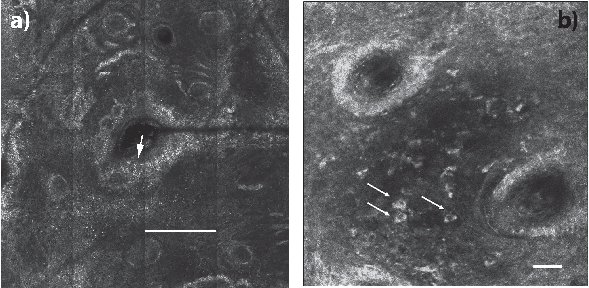
\includegraphics[width=0.8 \linewidth]{contents/x_microscopy/resources/example_rcm_pattern_3.pdf}
        \caption{Cas de données cliniques \gls{rcm} par Guitera~\cite{Guitera2010}. En a), exemple de cellules atypiques à proximité d'un follicule pileux au sein de la \gls{dej} sur un un \gls{lm}; En b), exemple de cellules nucléé du derme d'un \gls{lm}. Repère : barre = \SI{50}{\micro\metre}.}
        \label{fig:example_rcm_pattern_3}
    \end{center} 
\end{figure}\par

Dans l'étude menée par Cinotti~\cite{Cinotti2018}, les auteurs investigateurs ont demandés d'évaluer certaines caractéristiques récurrentes de la littérature. Parmis lesquelles:
\begin{itemize}
    \item Large roundish pagetoid cells. LM 37% (range 9-70%, SD 20), B 5% (range 1-13%, SD 4)
    \item large dendritic cells in the epidermis LM 81% (range 66-91%, SD 9), B  13% (range 8-20%, SD 4)
    \item follicular localization of atypical cells LM 62% (range 55-75%, SD 8), B 7% (range 3-11%, SD 2)
\end{itemize}\par

\begin{figure}[H]
    \begin{center}
        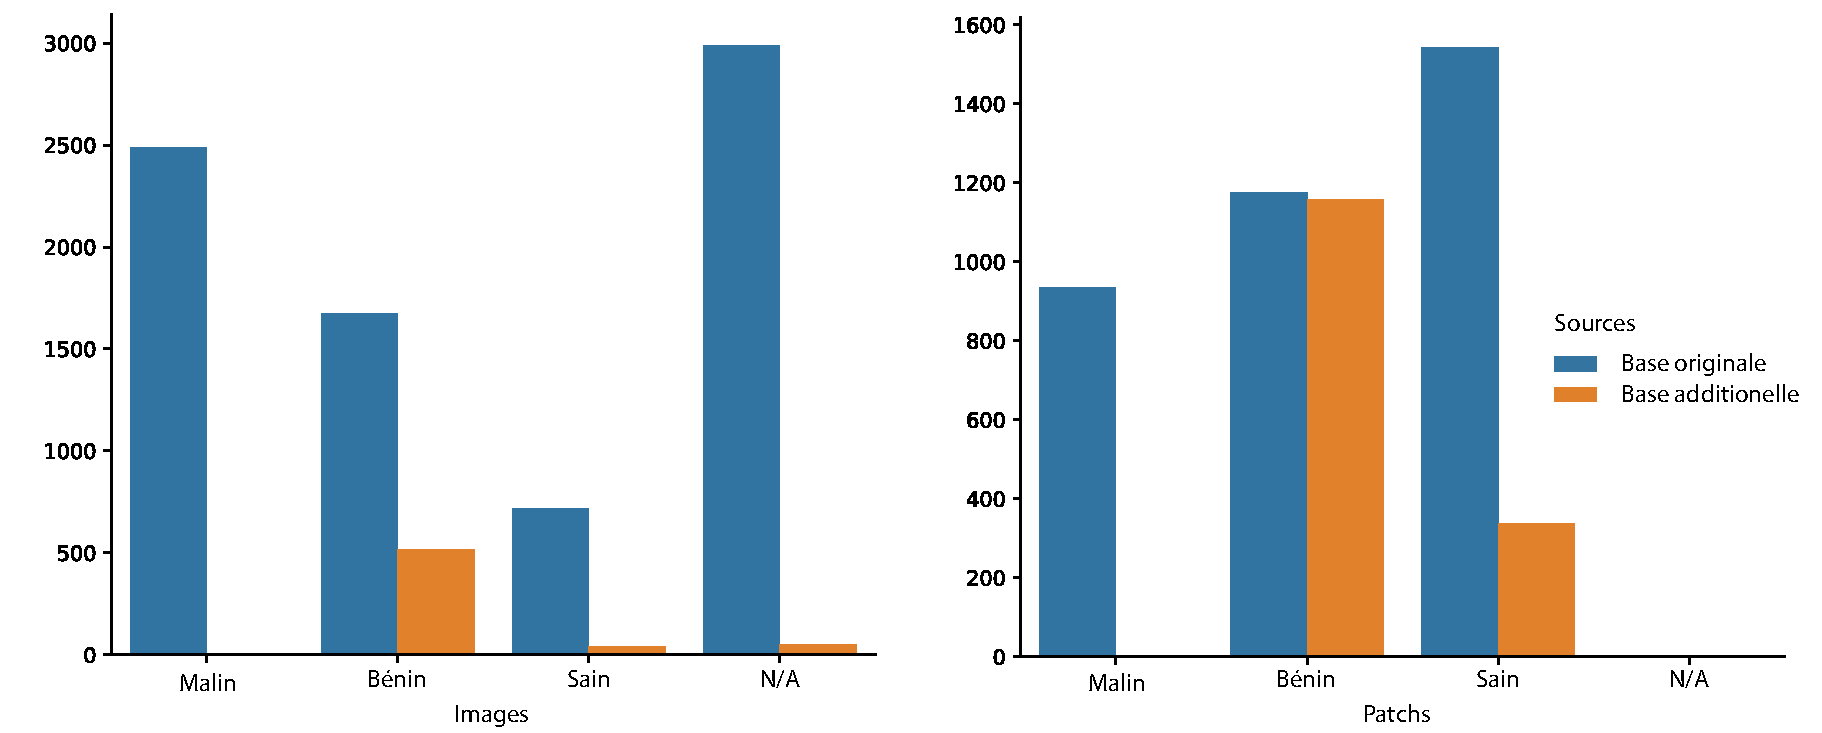
\includegraphics[width=\linewidth]{contents/x_microscopy/resources/scheme_rcm_statistics.pdf}
        \caption{Répartition de nos annotation au niveau des images (à gauche) mais également sur les patchs (à droite).}
        \label{fig:scheme_rcm_statistics}
    \end{center} 
\end{figure}\par

Les données \gls{rcm} de chaque lésions contiennent essentiellement des images jugées pertinentes par deux des trois médecins investigateurs et provenant de l'épiderme, de la \gls{dej} et du derme. Néanmoins, les données utilisées ici correspondront essentiellement à des données de la \gls{dej}. En effet, le \gls{lm}/\gls{lmm} sont des pathologies de la peau caractérisées par l'intrusion de de la mélanine se propageant le long des follicules pileux. Les images de la \gls{dej} sont ainsi parfaitement adaptées à l'observation de ce phénomène par les médecins. \par

Du point de vue de leurs caractéristique ces images arborent une taille constante de \SI{1000}{\px} $\times$ \SI{1000}{\px} pour une section mesurée de \SI{920}{\micro\metre} $\times$ \SI{920}{\micro\metre} pour une résolution axiale comprise entre \SIrange{3}{5}{\micro\metre}. Ces données fournissent ainsi une résolution de l'ordre du \SI{1}{\micro\metre}. De plus, aucune méta information ne pourra être utilisée pour traiter cette problématique, les quelques information étant pour la plupart erronée: procédure de calibration non réalisée, informations manquante, mode d'imagerie différents.\par

Pour finir, l'objectif visé par cette partie sera l'évaluation de technique d'imagerie sur la qualité du diagnostic sur base d'images issues de \gls{rcm}. A ce titre nous ne nous reposerons pas sur les méta données issues des informations patient: l'âge, le sexe ou encore l'emplacement seront autant de critères que nous ne considérerons pas au sein de ces prochains paragraphes bien que ceux ci soient utilisés par les dermatologues experts en \gls{rcm} durant leur évaluation~\cite{Cinotti2018}.\par

\begin{figure}[H]
    \begin{center}
        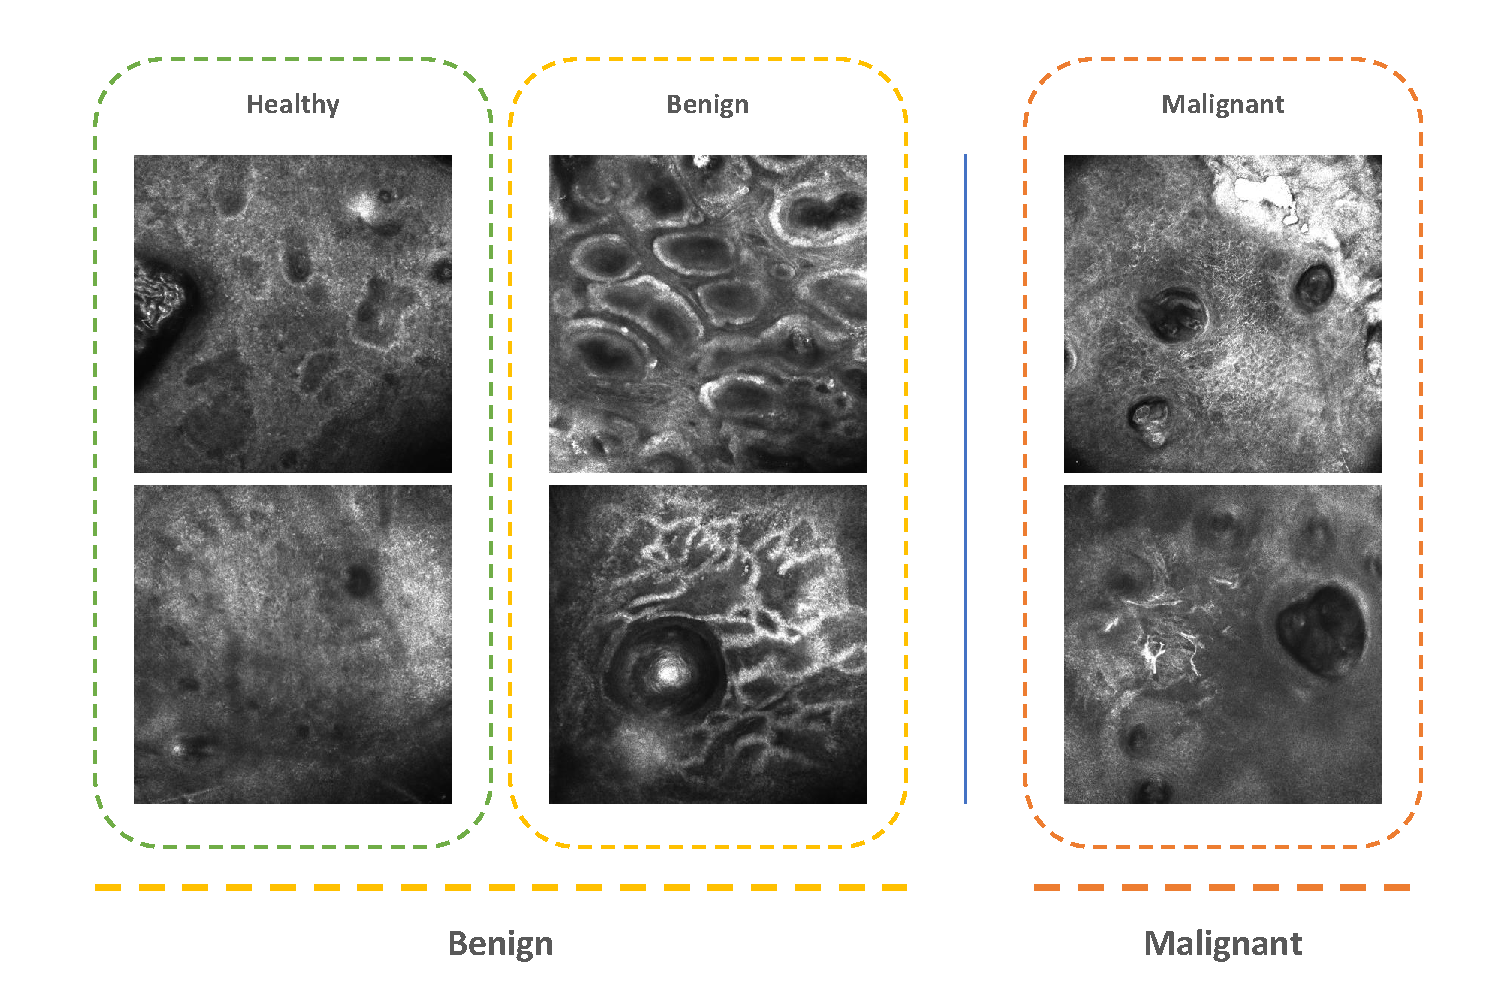
\includegraphics[width=\linewidth]{contents/x_microscopy/resources/example_rcm_data.pdf}
        \caption{Exemple de tissus.}
        \label{fig:example_rcm_data}
    \end{center} 
\end{figure}\par


Concernant l'étude de référence~\cite{Cinotti2018}, 
\begin{figure}[H]
    \begin{center}
        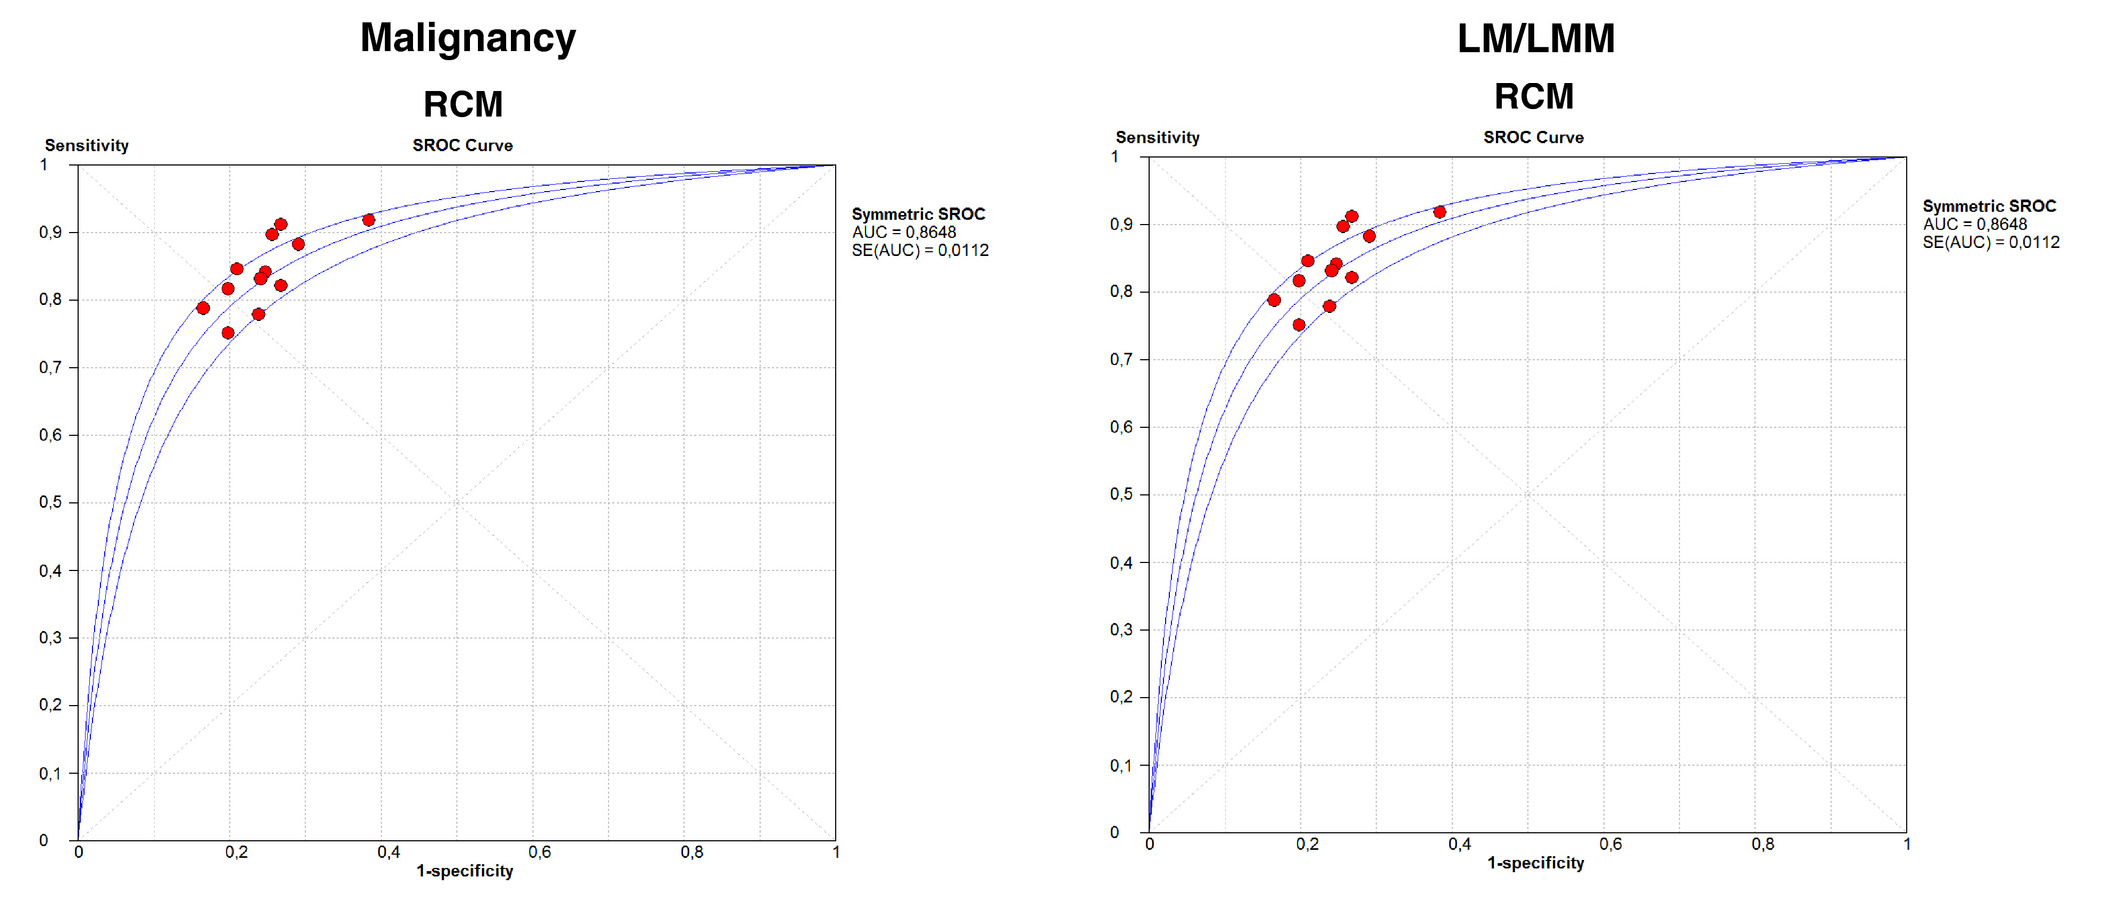
\includegraphics[width=\linewidth]{contents/x_microscopy/resources/results_rcm_experts.png}
        \caption{.}
        \label{fig:results_rcm_experts}
    \end{center} 
\end{figure}\par


Au sein de ce premier chapitre, nous élaborerons une méthodologie destinée à la modalité \gls{rcm}. Les éléments nous ayant conduit à nous intéresser à cette modalité sont multiples. En premier lieu, il s'agit de l'une des modalités les plus précise en notre possession, elle consiste donc en une référence en terme de qualité de diagnostic à réaliser. Enfin, le nombre restreint de travaux menée sur le diagnostic de lésion de la peau appliqué au \gls{rcm} assisté par ordinateur est un second argument. En effet, cette modalité représente pour nous un verrou scientifique nous devons lever pour accomplir le schéma de diagnostic multimodal.\par

Pour cela, nous sollicitons diverses ressources d'intelligence artificielle évoquées lors de précédent chapitre. De plus, certains ajouts ont été réalisés pour permettre le déroulement des expériences suivantes. En effet, la base d'image actuelle ne possède que des annotations au niveau des patients, ce qui limite fortement nos travaux.
A l'aide d'un outil graphique réalisé pour cette étude (\Cref{fig:example_gui_annotation}, nous avons pu obtenir grâce au travail de l'un des dermatologistes investigateur:
\begin{itemize}
\item des annotations au niveau des images,
\item des annotations au niveau de sous parties d'images ou \textbf{patchs}.
\end{itemize}\par

\begin{figure}[H]
\centering
    \begin{subfigure}{.45\textwidth}
      \centering
      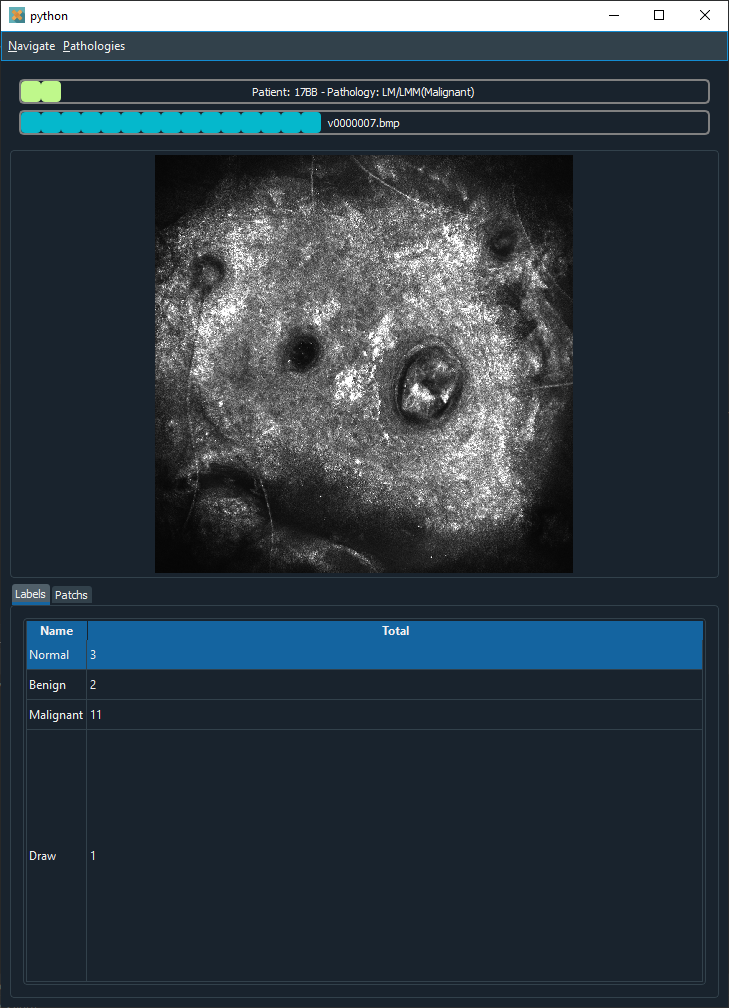
\includegraphics[width=0.8\linewidth]{contents/x_microscopy/resources/example_gui_annotation_1.png}
    \end{subfigure}
    \begin{subfigure}{.45\textwidth}
      \centering
      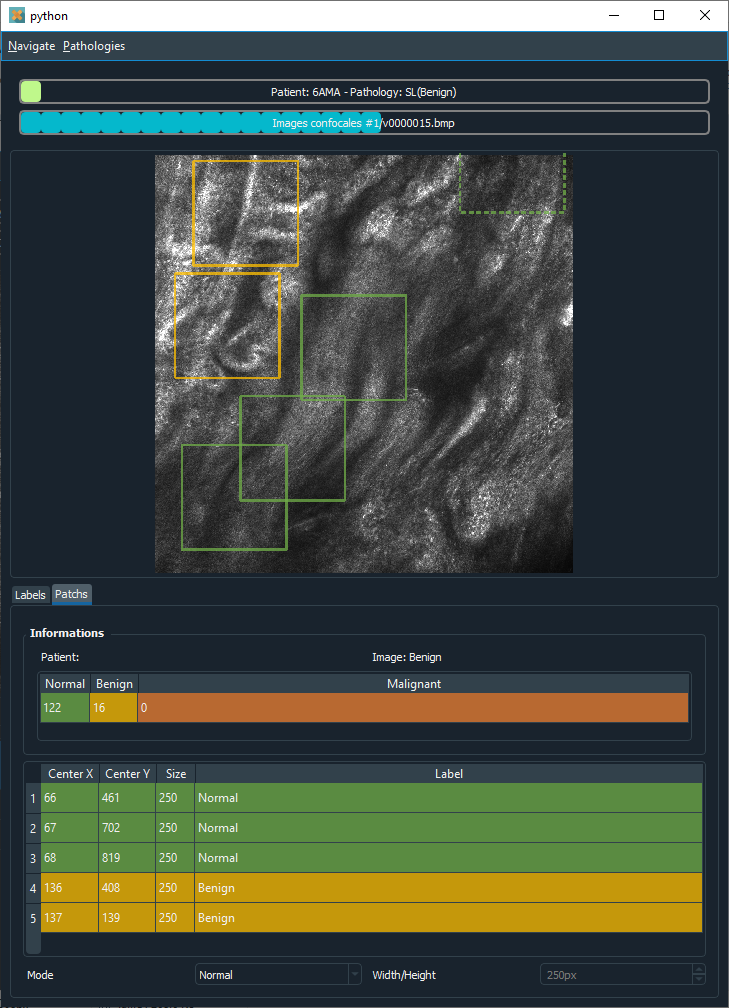
\includegraphics[width=0.8\linewidth]{contents/x_microscopy/resources/example_gui_annotation_2.png}
    \end{subfigure}
    \caption{Interface logicielle mise à disposition du spécialiste, afin de procédé aux annotations. A gauche, l'onglet permettant l'annotation au niveau des images, à droite l'onglet permettant la création de patchs.}
    \label{fig:example_gui_annotation}
\end{figure}

Ainsi, dans cette partie ne seront considérée que les données \gls{rcm} des 223 lésions en notre possession et seront donc exclues images de photographie clinique et dermatoscopie. Également, ont été utilisés 28 patient bénins non présent dans la base d'image initiale afin d'augmenter le nombre d'images annotées comme bénignes. Ces images comportent également des lésions pouvant porter à préjudice lors du diagnostic de \gls{lm}/\gls{lmm}. Ces données ne seront utilisées uniquement dans le but de renforcer l'entraînement. La répartition complète de cette base peux être visualisé en \Cref{fig:scheme_rcm_statistics}.\par


Afin de répondre à ce besoin, cette partie dédiée au \gls{rcm} se compose de trois chapitres dans lesquels nous élaborerons une méthodologie ascendante:
\begin{inlinerate}
\item le premier chapitre abordera la \textbf{prise de décision au niveau de l'image},
\item le second chapitre proposera des \textbf{perspectives d'amélioration},
\item enfin le dernier chapitre de cette section se focalisera sur une \textbf{prise de diagnostic au niveau du patient}.
\end{inlinerate}\par
\newpage